

\documentclass[11pt,a4paper, final, twoside]{article}
%%%%%%%%%%%%%%%%%%%%%%%%%%%%%%%%%%%%%%%%%%%%%%%%%%%%%%%%%%%%%%%%%%%%%%%%%%%%%%%%%%%%%%%%%%%%%%%%%%%%%%%%%%%%%%%%%%%%%%%%%%%%%%%%%%%%%%%%%%%%%%%%%%%%%%%%%%%%%%%%%%%%%%%%%%%%%%%%%%%%%%%%%%%%%%%%%%%%%%%%%%%%%%%%%%%%%%%%%%%%%%%%%%%%%%%%%%%%%%%%%%%%%%%%%%%%
\usepackage{amsmath}
\usepackage{fancyhdr}
\usepackage{amsthm}
\usepackage{amsfonts}
\usepackage{amssymb}
\usepackage{amscd}
\usepackage{latexsym}
\usepackage{graphicx}
\usepackage{graphics}
\usepackage{natbib}
\usepackage[colorlinks=true, urlcolor=blue,  linkcolor=black, citecolor=black]{hyperref}
\usepackage{color}
\usepackage{natbib}
\usepackage{sectsty}
\setcounter{MaxMatrixCols}{10}


\sectionfont{\fontsize{12}{15}\selectfont}

\renewcommand{\thefootnote}{}
\setlength{\oddsidemargin}{1pt} \setlength{\evensidemargin}{1pt}
\setlength{\hoffset}{-1in} \addtolength{\hoffset}{25mm}
\setlength{\textwidth}{140mm} 
\setlength{\marginparsep}{0pt} \setlength{\marginparwidth}{0pt}
\setlength{\topmargin}{0pt}
\setlength{\voffset}{-2in} \addtolength{\voffset}{20mm}
\setlength{\textheight}{250mm}
\setlength{\headsep}{20mm}
\setlength{\footskip}{15mm}
\pagestyle{fancy}
\fancyhead{} \fancyfoot{} 



%       Theorem environments
\newtheorem{thm}{Theorem}[section]
\newtheorem{algorithm}[thm]{Algorithm}
\newtheorem{axiom}[thm]{Axiom}
\newtheorem{lem}[thm]{Lemma}
\newtheorem{example}[thm]{Example}
\newtheorem{exercise}[thm]{Exercise}
\newtheorem{notation}[thm]{Notation}
\newtheorem{problem}[thm]{Problem}
\theoremstyle{proposition}
\newtheorem{prop}{Proposition}[section]
\newtheorem{case}[thm]{Case}
\newtheorem{claim}[thm]{Claim}
\newtheorem{conclusion}[thm]{Conclusion}
\newtheorem{condition}[thm]{Condition}
\newtheorem{conjecture}[thm]{Conjecture}
\newtheorem{cor}[thm]{Corollary}
\newtheorem{criterion}[thm]{Criterion}
\theoremstyle{definition}
\newtheorem{defn}{Definition}[section]
\theoremstyle{remark}
\newtheorem{rem}{Remark}[section]
\newtheorem{solution}[thm]{Solution}
\newtheorem{summary}[thm]{Summary}
\numberwithin{equation}{section}
\renewcommand{\rmdefault}{phv} % Arial
\renewcommand{\sfdefault}{phv} % Arial
\pagenumbering{arabic} % 1, 2, 3, 4, ...

%%%%%%%%%%%%%%%%%%%%%%%%%%%%%%%%%%%%%%%%%%%%%%%%%%%%%%%%%%%%

% non-template additions

\usepackage{caption}
\usepackage[margin=.7cm]{subcaption}

\setlength{\parindent}{0pt}
\setlength{\parskip}{1em}

%%%%%%%%%%%%%%%%%%%%%%%%%%%%%%%%%%%%%%%%%%%%%%%%%%%%%%%%%%%%

\begin{document}
\hyphenpenalty=100000

\begin{center}

{\Large \textbf{\\Geodesicness for Meshfree Simulation Methods }}\\[5mm]
{\large \textbf{Darren Moore}\\[1mm]}
{\normalsize \emph{Under the supervision of Professor David I.W. Levin and Professor Alec Jacobson}\\[1mm]}
\end{center}

\section{Introduction}
Elasticity simulation can be used to animate the clothes that CGI characters wear or calculate how much weight structures will hold before they collapse \cite{Irving:2004:IFE:1028523.1028541} \cite{Clough:1990:OFF:106419.106421}. In general it lets us model how objects deform when forces are applied to them. The numerical methods used to do this require the object we're simulating to be discretized into finite pieces. The technique by which we discretize the object gives rise to two classes of numerical methods. One class, called Finite Element Methods, uses a polygon mesh discretization (Figure \ref{fig:meshA}), but mesh generation requires a lot of user tuning and can fail if the object has complicated geometry. The other class is Meshfree Methods, which uses a point cloud discretization (Figure \ref{fig:meshB}) rather than a mesh to perform the simulation.

\begin{figure}[h]
\centering
\begin{subfigure}[t]{.5\textwidth}
  \centering
  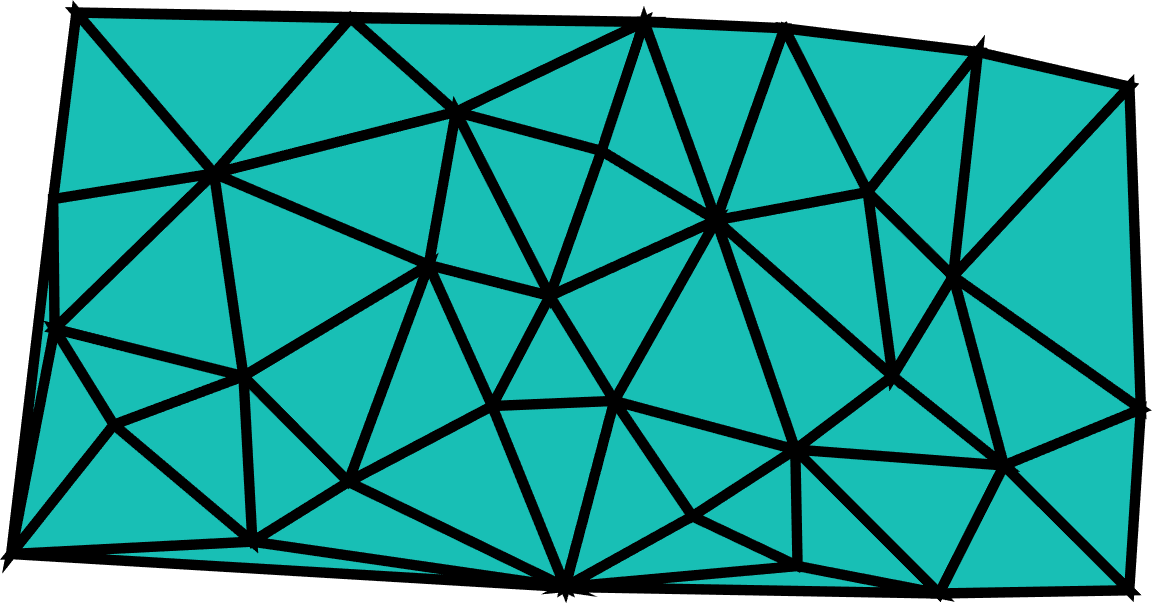
\includegraphics[width=.7\linewidth]{meshEx.png}
  \caption{A triangle mesh for the finite element method.}
    \label{fig:meshA}
\end{subfigure}%
\begin{subfigure}[t]{.5\textwidth}
  \centering
  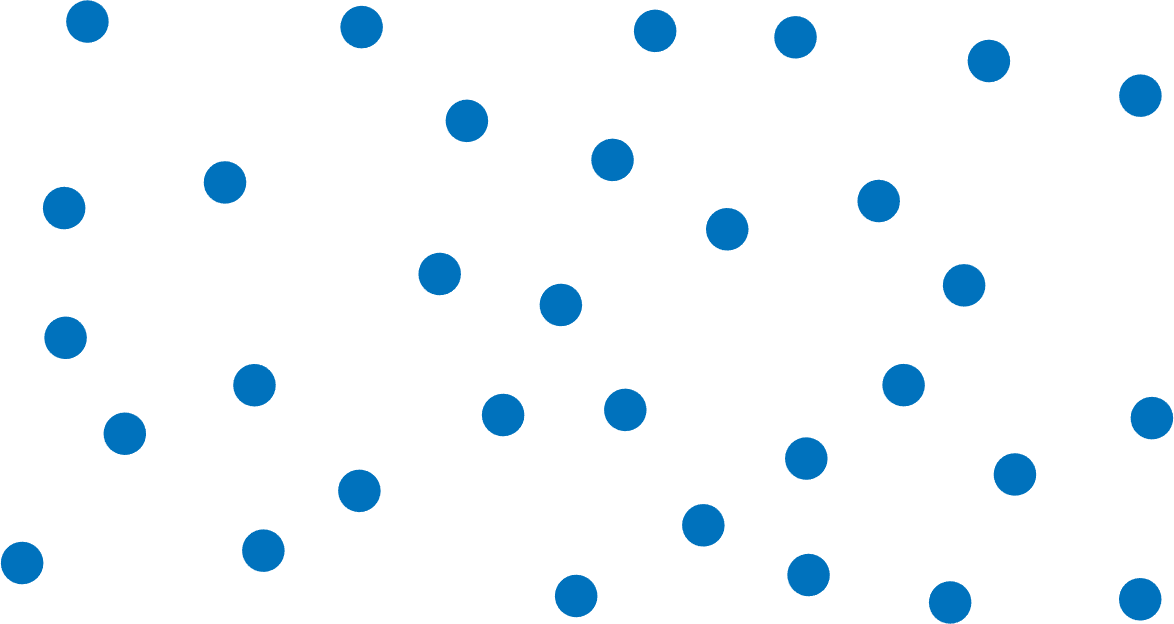
\includegraphics[width=.7\linewidth]{meshFreeEx.png}
  \caption{A point cloud for meshfree methods.}
    \label{fig:meshB}
\end{subfigure}
\caption{Two discretizations of an object that can be used for simulation.}
\label{fig:mesh}
\end{figure}

An important distinction between point cloud and polygon mesh representations is the point cloud's lack of connectivity information. Elasticity requires a notion of connectivity to determine how applying a force to one point affects the points connected to it. Most meshfree methods simply take the set of all points in a certain radius $h$ around a given point to be connected to it (Figure \ref{fig:radius}). \cite{liu2005introduction} 

\begin{figure}[h]
\centering
\begin{subfigure}[t]{.5\textwidth}
  \centering
  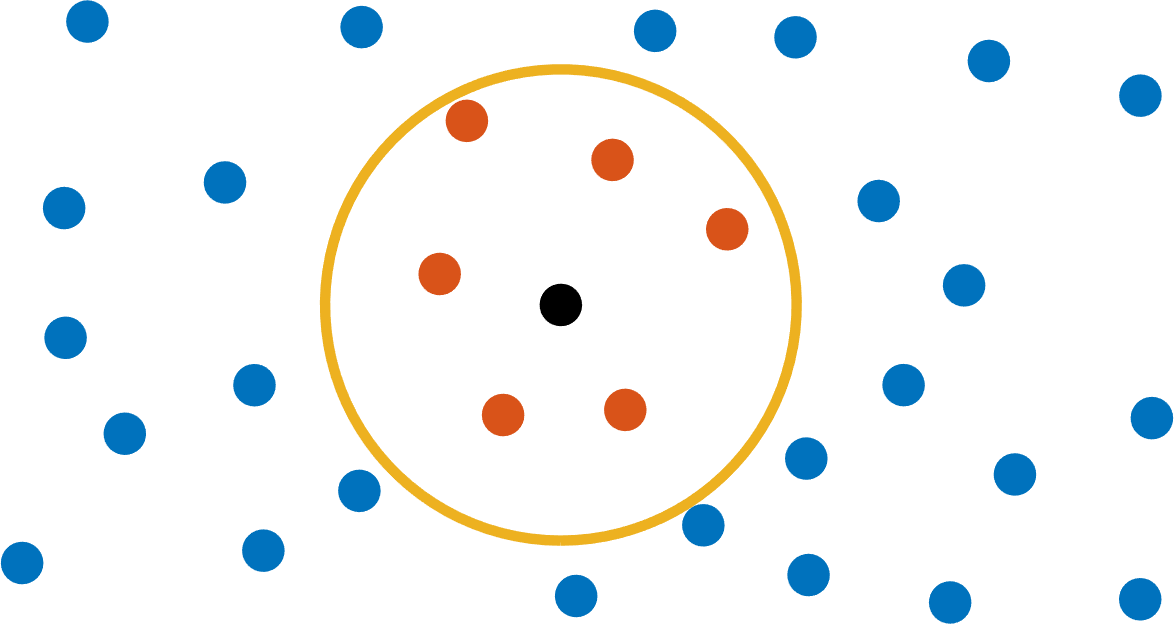
\includegraphics[width=.7\linewidth]{smallRadius.png}
  \caption{All points in a radius $h$ are connected.}
\end{subfigure}%
\begin{subfigure}[t]{.5\textwidth}
  \centering
  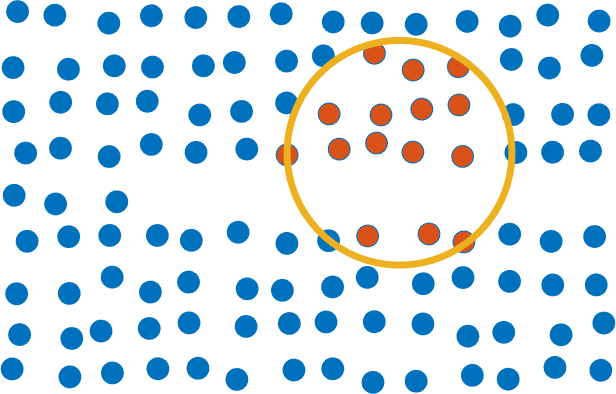
\includegraphics[width=.7\linewidth]{badRadius.png}
  \caption{A case where the radial approach connects across a gap.}
\end{subfigure}
\caption{The radial approach in meshfree methods.}
\label{fig:radius}
\end{figure}

This radial approach is problematic if two points are close to each other in space but have a large geodesic distance. Geodesic distance is the shortest distance between two points when taking paths that stay on the object (Figure \ref{fig:geodesic}). An incorrect interpretation of the topology will result in ``invisible connections'' that incorrectly constrain the movement of the object (Figure \ref{fig:geoBad}). The goal of our paper is to enhance the interpretation of the topology using point cloud geodesics. If you think of the point cloud as approximating a 2D shape, then a point cloud geodesic between two points is the geodesic distance between the points lying that 2D shape.

\begin{figure}[h]
\centering
\begin{subfigure}[t]{.5\textwidth}
  \centering
  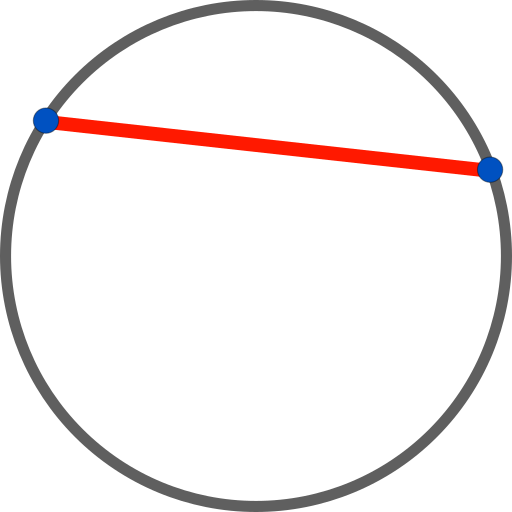
\includegraphics[width=.5\linewidth]{distancesEuch.png}
  \caption{Euclidean distance cuts through space.}
\end{subfigure}%
\begin{subfigure}[t]{.5\textwidth}
  \centering
  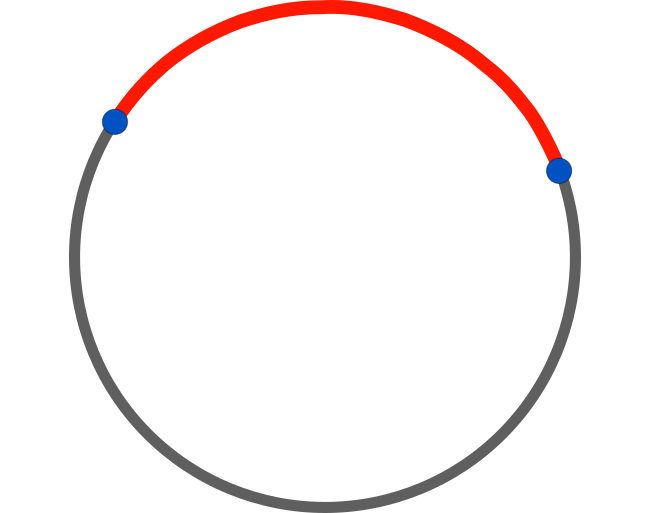
\includegraphics[width=.5\linewidth]{distanceGeo.png}
  \caption{Geodesic distance stays on the object.}
\end{subfigure}
\caption{The Euclidean distance vs. geodesic distance between two points on a circle.}
\label{fig:geodesic}
\end{figure}

\begin{figure}[h]
\centering
\begin{subfigure}[t]{.5\textwidth}
  \centering
  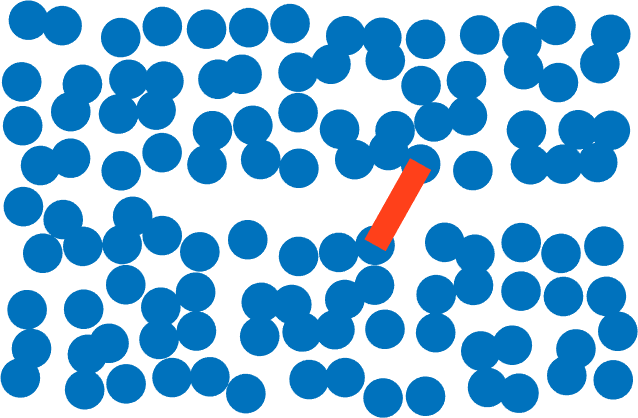
\includegraphics[width=.7\linewidth]{jumpLine.png}
  \caption{}
\end{subfigure}%
\begin{subfigure}[t]{.5\textwidth}
  \centering
  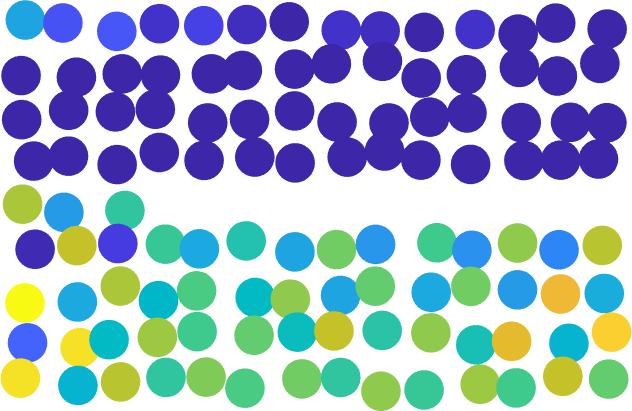
\includegraphics[width=.7\linewidth]{pantsStay.png}
  \caption{}
\end{subfigure}
\caption{Due to an ``invisible connection'' in (a), the movement of the object is incorrectly constrained in (b). We expect the elastic lower bar to bend downwards.}
\label{fig:geoBad}
\end{figure}


\section{Approach}

We combine meshfree methods with point cloud geodesics to more accurately simulate point cloud data. The core of our approach is to use shortest-path graph searches to compute point cloud geodesic distances, then simulating the particles using those geodesic distances rather than standard Euclidean distances.

To compute these point cloud geodesic distances, we represent the point cloud as a weighted graph with edge weights equal to the Euclidean distance between points (Figure \ref{fig:graph}). By exponentiating the weights we penalize large jumps. With sufficiently large exponent, the shortest-path graph distance approximates the geodesic distance.


\begin{figure}[h]
\centering
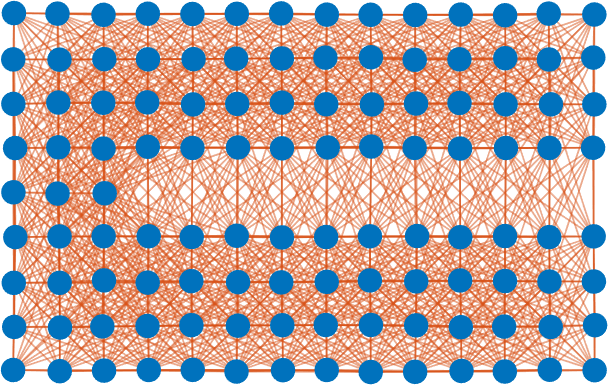
\includegraphics{pointGraph.png}
\caption{A graph defined over a point cloud. Two points are connected by an edge when their Euclidean distance is less than or equal to $h$. Edge weights are not represented in this figure.}
\label{fig:graph}
\end{figure}

We define our graph as follows: given points $x_i$ and $x_j$, $(x_i, x_j)$ is an edge if and only if $\|x_i - x_j\| \leq h$, where $\|\cdot\|$ is the Euclidean norm. While our methods work if the graph is complete, we only connect points in a small radius to increase efficiency. Denote the edge weights by $w(x_i,x_j)$.

We define a parameter, the \textit{geodesicness}, which represents the extent to which our method avoids large jumps while searching for a geodesic path between points. Let $\gamma \geq 1.0$ denote the geodesicness. Different point clouds may require different values of $\gamma$ since there will be different sized jumps in the data. This parameter is tuned by the user.

Our geodesic approach uses $w(x_i, x_j) = \|x_i - x_j\|^\gamma$. As a result, large jumps in the data are expensive for the shortest-path graph search. With a sufficiently large $\gamma$, the path will walk around gaps and take a point cloud geodesic path (Figure \ref{fig:geoWalk}). It can be seen that letting $\gamma = 1.0$ is equivalent to the traditional approach. The geodesicness required to get an improved simulation result depends on the size of the gaps in the data, the number of points along the geodesic paths, and the distance between each point along the geodesic paths.

\begin{figure}[h]
\centering
\begin{subfigure}[t]{.5\textwidth}
  \centering
  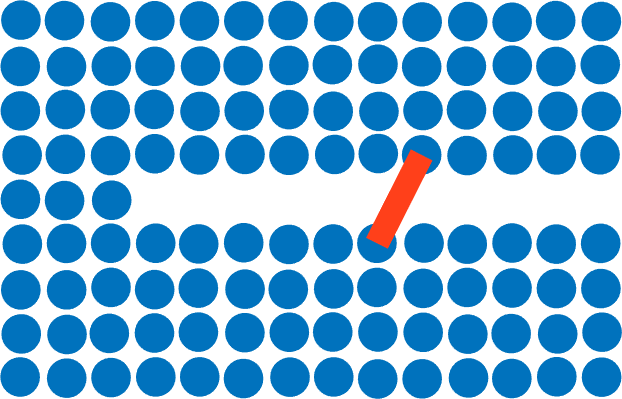
\includegraphics[width=.7\linewidth]{jumpLineGrid.png}
  \caption{Regular grid of particles.}
\end{subfigure}%
\begin{subfigure}[t]{.5\textwidth}
  \centering
  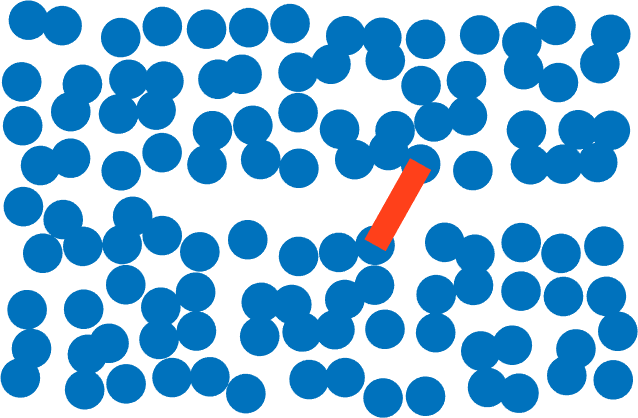
\includegraphics[width=.7\linewidth]{jumpLine.png}
  \caption{Noisy particle arrangement.}
\end{subfigure}

\caption{The shortest path with a traditional radial based approach.}
\label{fig:jump}
\end{figure}

\begin{figure}[h]
\centering
\begin{subfigure}[t]{.5\textwidth}
  \centering
  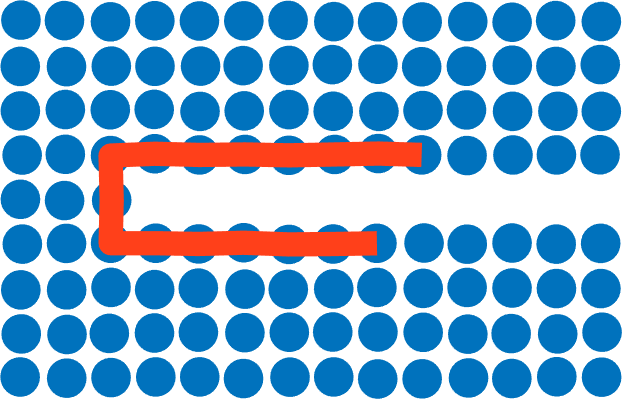
\includegraphics[width=.7\linewidth]{geodesicLineGrid.png}
  \caption{Regular grid of particles.}
\end{subfigure}%
\begin{subfigure}[t]{.5\textwidth}
  \centering
  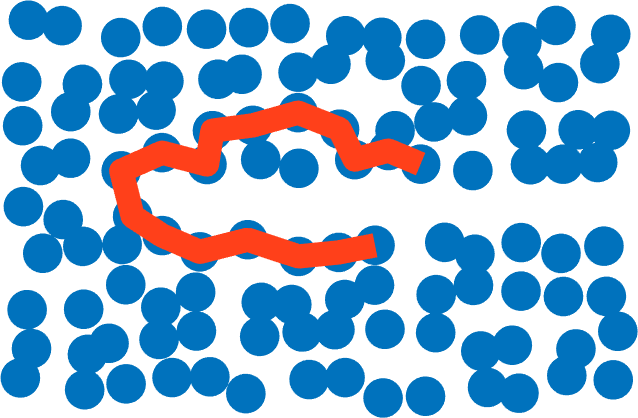
\includegraphics[width=.7\linewidth]{geodesicLine.png}
  \caption{Noisy particle arrangement.}
\end{subfigure}
\caption{The shortest path with our geodesic approach.}
\label{fig:geoWalk}
\end{figure}


\section{Results}


We demonstrate our method's effectiveness by applying it to several point cloud data sets. Our simulations were done using a linear elastic material model, although our method works independently of the material model.

Figure \ref{fig:barDrop} uses a point cloud of two bars connected only on the left. We fix the top bar in place and leave the bottom bar free to deform under gravity. With the traditional radial approach, the bottom bar does not deform, since it is incorrectly connected to the fixed top bar. With our geodesic approach, the bottom bar is free to bend downwards.

\begin{figure}[h]
\centering
\begin{subfigure}[t]{.5\textwidth}
  \centering
  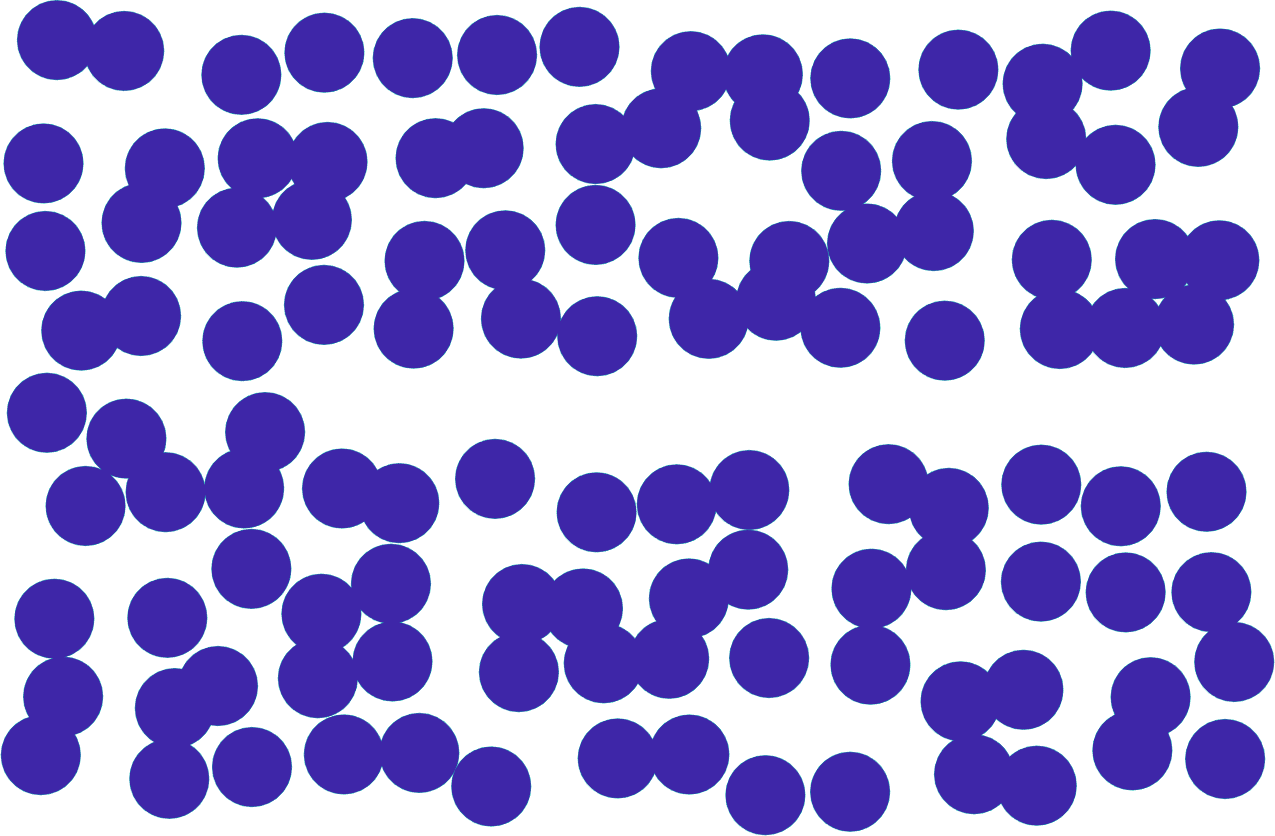
\includegraphics[width=.7\linewidth]{blockUndef.png}
  \caption{An undeformed point cloud.}
\end{subfigure}%

\includegraphics[scale=.25]{parula.png}

\begin{subfigure}[t]{.5\textwidth}
  \centering
  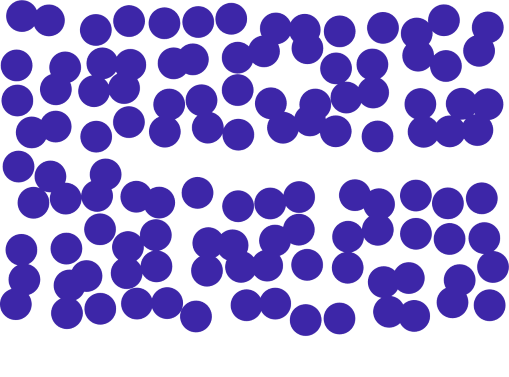
\includegraphics[width=.7\linewidth]{pantsStayColor.png}
  \caption[width=2\textwidth]{Traditional radial approach: No visible deformation.}
\end{subfigure}%
\begin{subfigure}[t]{.5\textwidth}
  \centering
  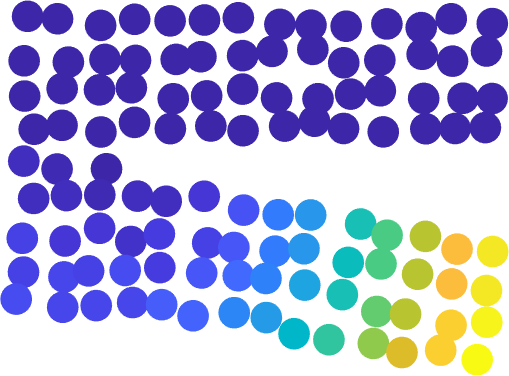
\includegraphics[width=.7\linewidth]{pantsFall.png}
  \caption{Our geodesic approach: The bar bends downwards as expected. Uses $\gamma = 15$.}
\end{subfigure}
\caption{The upper bar is held in place while an elastic lower bar should bend down due to gravity. Colour denotes displacement from original position.}
\label{fig:barDrop}
\end{figure}

Figure \ref{fig:pantsKick} demonstrates our approach in the case of a user interacting with a pair of point cloud pants. We begin by fixing the top of the pants in place and allow the legs to deform freely. Next, a user attempts to pull the right leg to the right. With the traditional radial approach, the legs are incorrectly connected together and both pant legs deform. With our geodesic approach, the legs can move independently of each other as expected.

\begin{figure}[h]
\centering
\begin{subfigure}[t]{.5\textwidth}
  \centering
  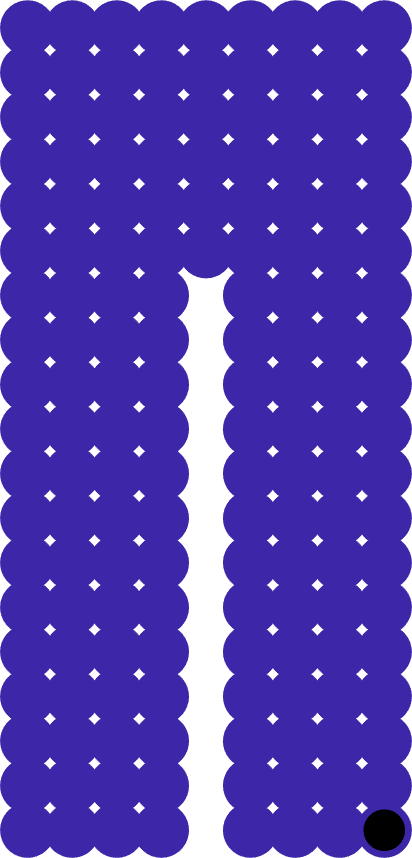
\includegraphics{pantsUndefColor.png}
  \caption{An undeformed point cloud of a pair of pants.}
\end{subfigure}%

\includegraphics[scale=.25]{parula.png}
\begin{subfigure}[t]{.5\textwidth}
  \centering
  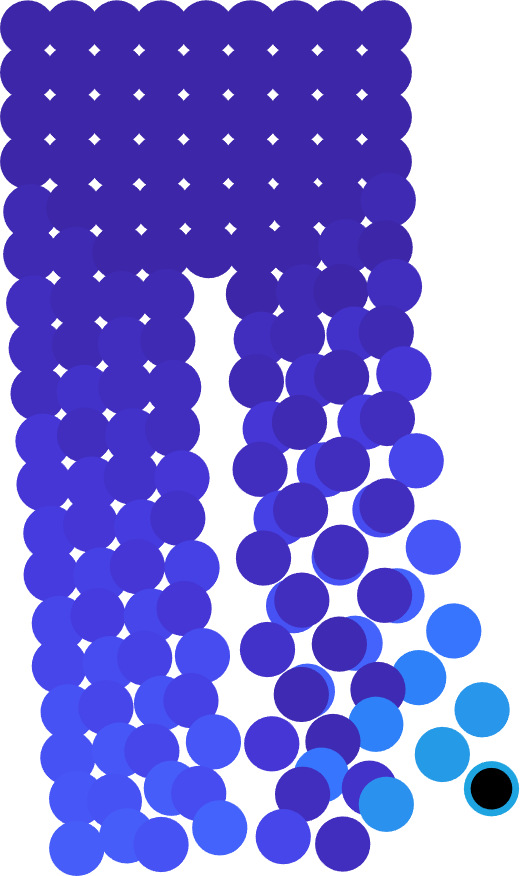
\includegraphics{pantsLongStayColor.png}
  \caption{Traditional radial approach: The legs are stuck together.}
\end{subfigure}%
\begin{subfigure}[t]{.5\textwidth}
  \centering
  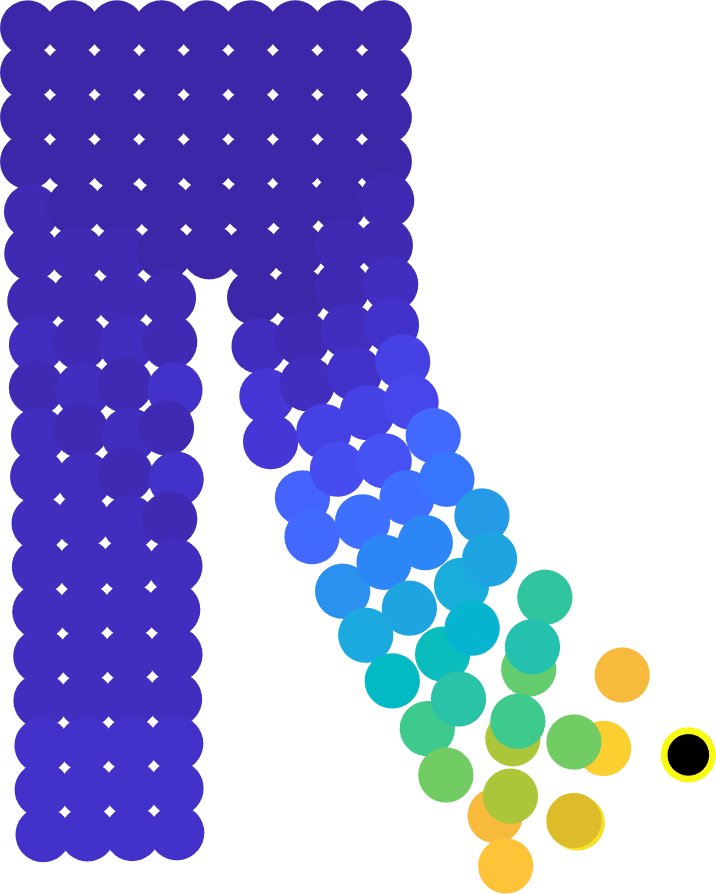
\includegraphics{pantsKickColor.png}
  \caption{Our geodesic approach: The artificial constraint is not present. Uses $\gamma = 15$.}
\end{subfigure}
\caption{A user deforms a pair of pants by pulling the black particle to the right. Colour denotes displacement from original position.}
\label{fig:pantsKick}
\end{figure}

Figure \ref{fig:octopusBandit} demonstrates an application of our approach to character animation. We begin by fixing the head of the octopus in place and allow the arms to deform freely. With the traditional approach, the animator can't wiggle the arms around as they are stuck together. With our geodesic approach, the arms can move independently, allowing the octopus to wave hello.

\begin{figure}[h]
\centering
\begin{subfigure}[t]{.5\textwidth}
  \centering
  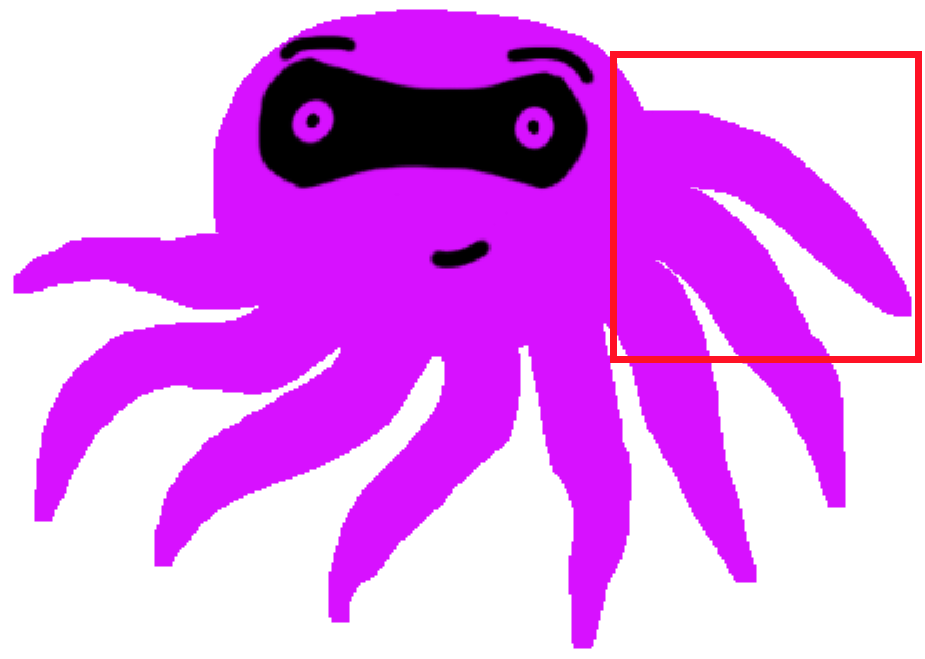
\includegraphics[width=.9\linewidth]{octoUndefRed.png}
  \caption{The undeformed octopus bandit.}
\end{subfigure}
\begin{subfigure}[t]{.5\textwidth}
  \centering
  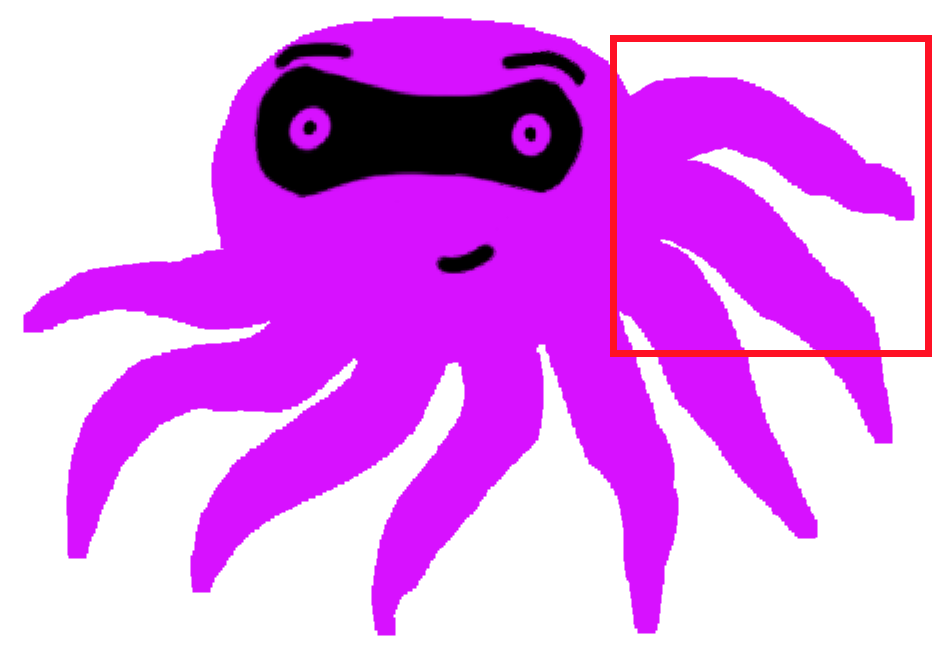
\includegraphics[width=.9\linewidth]{octoConnectRed.png}
  \caption{Traditional radial approach: The arms are stuck together.}
\end{subfigure}%
\begin{subfigure}[t]{.5\textwidth}
  \centering
  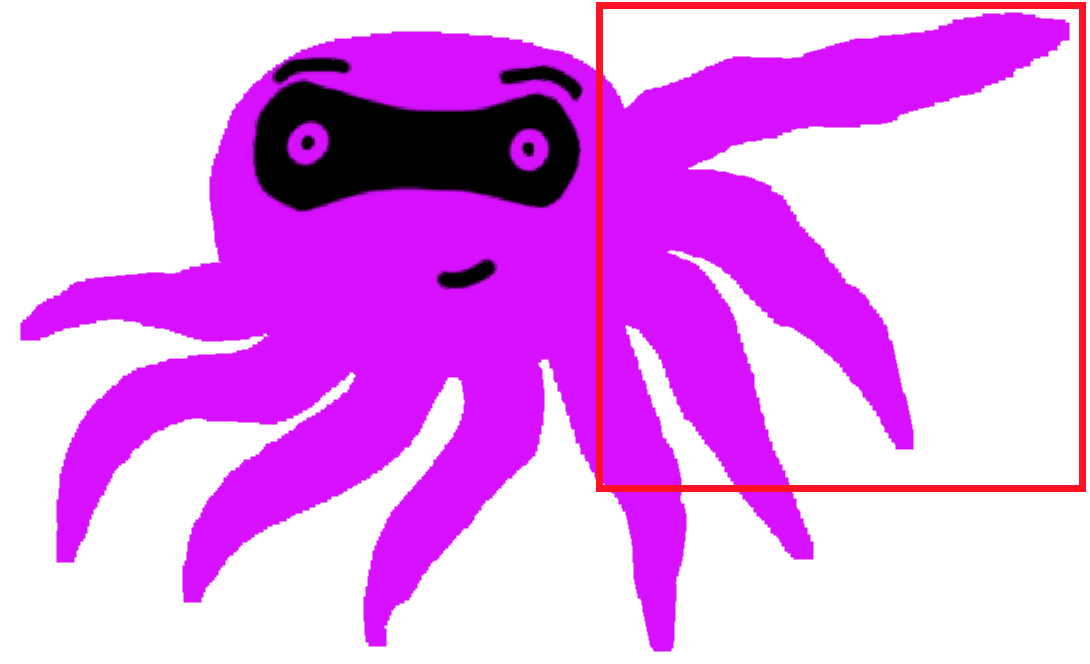
\includegraphics[width=1\linewidth]{octoHelloRed.png}
  \caption{Our geodesic approach: The arms may move freely. Uses $\gamma = 15$.}
\end{subfigure}
\caption{An artist attempts to animate the octopus bandit waving hello.}
\label{fig:octopusBandit}
\end{figure}



\section{Limitations}

Unfortunately, the quality of a simulation produced using this method does not gracefully degrade as the geodesicness decreases. If the geodesicness falls below a certain threshold, the close points that are far geodesically will immediately connect and the simulation will behave as in the traditional radial approach.

\section{Conclusion}
Since point clouds have no connectivity information it's easy to incorrectly interpret the topology when simulating elasticity. We introduced a method which combines meshfree methods with point cloud geodesics to help interpret the topology in cases where points are close in space but far geodesically. Future work includes generalizing to three dimensions and investigating a gracefully degrading point cloud geodesic distance.

\mbox{}\\

\noindent \Large\textbf{Acknowledgement}\\[1mm]
\normalsize \noindent I would like to acknowledge David Levin and Alec Jacobson, my supervisors, and Tim Jeruzalski, my mentor, for their support and ideas throughout this project.\\[3mm]

\bibliography{refs.bib}
\bibliographystyle{plain}

\end{document}
